\numberwithin{equation}{section}

\subsection{Nondimensionalization}
%\begin{frame}
  %\frametitle{Outline}
  %\tableofcontents[ currentsection ]
%\end{frame}

\begin{frame}
\frametitle{Nondimensionalization}

  The nondimensionalized system is:

	\begin{align*}
		\frac{dx}{dt} &= x^2 (1-x) - \alpha xy - \frac{\gamma_\circ x^2}{x+D}, \\
    \frac{dy}{dt} &= \rho y^2 (1-y) - \beta xy -\frac{\delta_\circ y^2}{y+R}
	\end{align*}
\end{frame}

\begin{frame}{Phase Plane}

  \vfill


  
  \begin{columns}
    \only<1> {
      \column{.65\textwidth}
      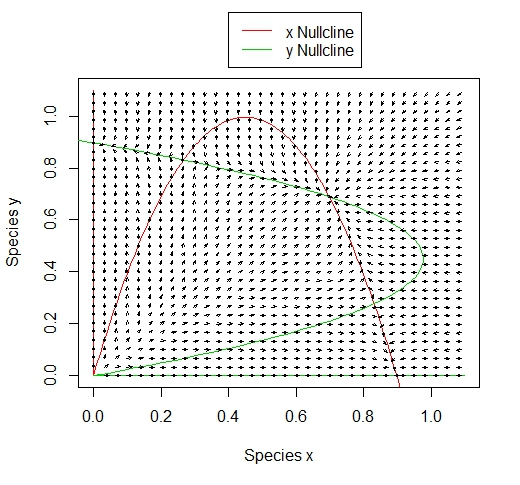
\includegraphics[height=7cm]{img/RplotMain}
      \column{.35\textwidth}
      $\alpha = .2, \beta = .2,
      \gamma = .8, \delta = .4, \rho = 1, R = 3$ and $D = 7$ 

      \begin{itemize}
      \item Six fixed points.
      \item Three are unstable.
      \end{itemize}
    }

    \only<2> {
      \column{.65\textwidth}
      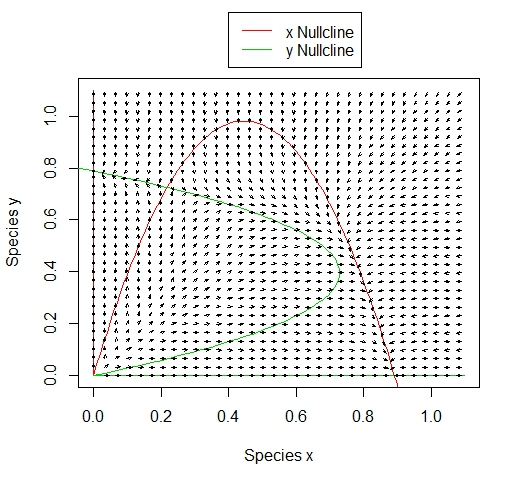
\includegraphics[height=7cm]{img/Rplot1} 
      \column{.35\textwidth}
      $\gamma = .85$ and $\delta = .8$ 
      \begin{itemize}
      \item Four fixed points.
      \item Two are unstable.
      \end{itemize}
    }

    \only<3> {
      \column{.65\textwidth}
      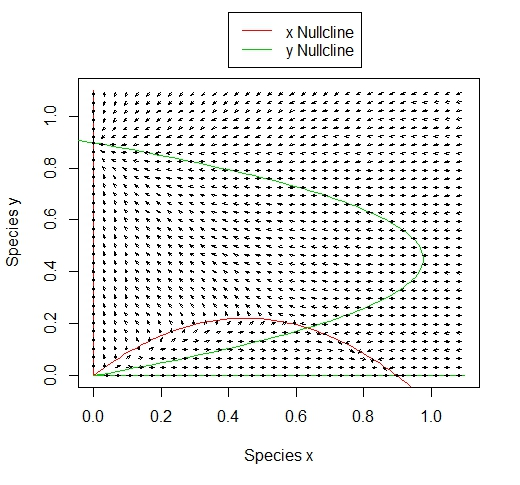
\includegraphics[height=7cm]{img/Rplot2} 
      \column{.35\textwidth}
      $\alpha = .9, \beta = .2, \gamma = .8$ and $\delta = .4$
      \begin{itemize}
      \item Four fixed points.
      \item Two are unstable.
      \end{itemize}
    }

    \only<4> {
      \column{.65\textwidth}
      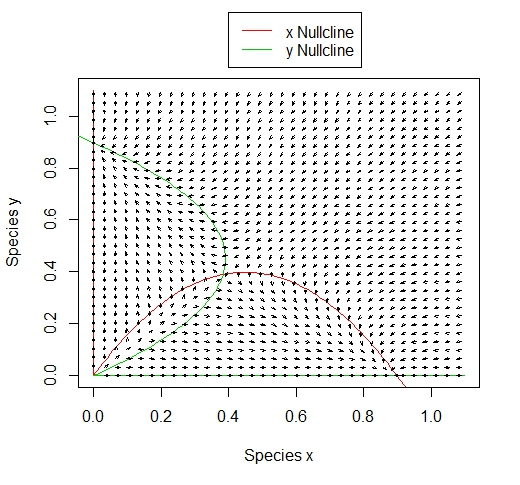
\includegraphics[height=7cm]{img/Rplot3} 
      \column{.35\textwidth}
      $\alpha = .5, \beta = .5, \gamma = .8$ and $\delta = .4$ 
      \begin{itemize}
      \item Four fixed points.
      \item Two are unstable.
      \end{itemize}
    }

    \only<5> {
      \column{.65\textwidth}
      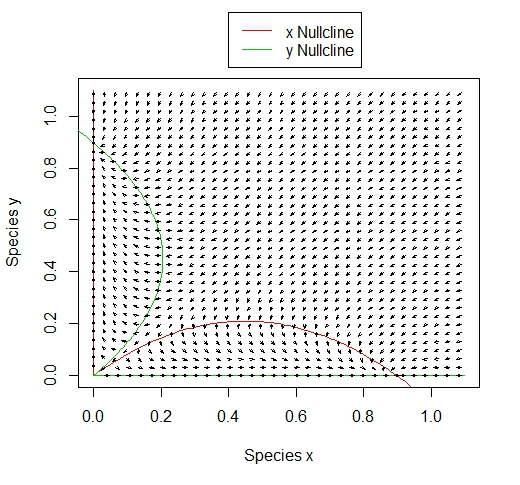
\includegraphics[height=7cm]{img/Rplot4} 
      \column{.35\textwidth}
      $\alpha = .95, \beta = .95, \gamma = .8$ and $\delta = .4$ 
      \begin{itemize}
      \item Three fixed points.
      \item Two are unstable.
      \end{itemize}
    }

  \end{columns}
\end{frame}




\begin{frame}{Noise}

  Additive noise...
  \begin{align*}
    \frac{dx}{dt} &= x^2 (1-x) - \alpha xy - \frac{\gamma_\circ x^2}{x+D} + \upsilon \frac{dW}{dt}, \\
    \frac{dy}{dt} &= \rho y^2 (1-y) - \beta xy -\frac{\delta_\circ y^2}{y+R}+ \kappa \frac{dB}{dt}.
  \end{align*}

  Proportional noise...
  \begin{align*}
    \frac{dx}{dt} &= x^2 (1-x) - \alpha xy - \frac{\gamma_\circ x^2}{x+D} + \upsilon x \frac{dW}{dt}, \\
    \frac{dy}{dt} &= \rho y^2 (1-y) - \beta xy -\frac{\delta_\circ y^2}{y+R}+ \kappa y \frac{dB}{dt}.
  \end{align*}

\end{frame}




\begin{frame}
\frametitle{Heun's Method}
\begin{itemize}
\item Heun's method is a numerical procedure for approximating ordinary differential equations with a given initial value.
\item First you calculate the intermediate value $\tilde{y}_{i+1}$ and then the final approximation $y_{i+1}$ at the next generation point.
\end{itemize}

\begin{align*}
	\tilde{y}_{i+1} &= y_i + \Delta t \ f(t_i, y_i) \\
	y_{i+1} &= y_i + \frac{\Delta t}{2} \left[f(y_i,t_i) + f(\tilde{y}_{i+1}, t_{i+1})\right]
\end{align*}
\end{frame}


\begin{frame}
   \frametitle{Heun's Method vs. Euler's Method - Simulation}
For the DE $y'=r y$ on $[0,T]$,\\
\vspace{1em}
	%\hspace{1.5em} Heun's:$\hspace{1em} \tilde{y}_{i+1} = y_i + \Delta t \ f(t_i, y_i)$ \\
		\hspace{1.5em} Heun's:$ \hspace{1em} y_{i+1} = y_i + \frac{\Delta t}{2} \left[f(y_i,t_i) + f(\tilde{y}_{i+1}, t_{i+1})\right]$ \vspace{1em} \\
	\hspace{1.5em} Euler's:$\hspace{1em}\tilde{y}_{i+1} = y_i + \Delta t \ f(y_i, t_i)$ \\
\begin{columns}[t]
    \column{.5\textwidth} 
    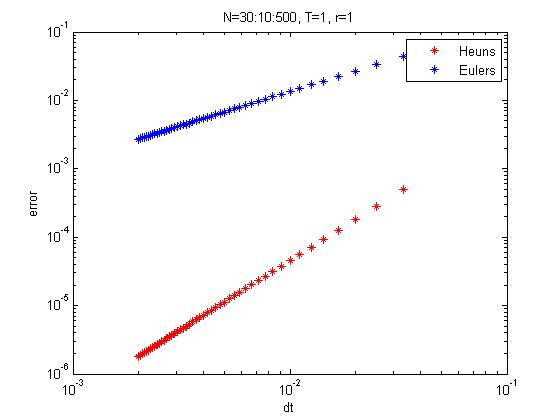
\includegraphics[width=6cm]{img/Heun500}
    \column{.5\textwidth}
    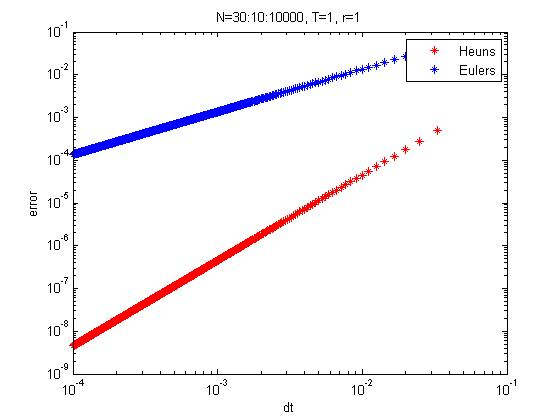
\includegraphics[width=6cm]{img/Heun10000}
  \end{columns}

\end{frame}
